% Options for packages loaded elsewhere
\PassOptionsToPackage{unicode}{hyperref}
\PassOptionsToPackage{hyphens}{url}
%
\documentclass[
]{article}
\title{Estimando los Parametros}
\author{BIOL4558}
\date{Agosto 2021}

\usepackage{amsmath,amssymb}
\usepackage{lmodern}
\usepackage{iftex}
\ifPDFTeX
  \usepackage[T1]{fontenc}
  \usepackage[utf8]{inputenc}
  \usepackage{textcomp} % provide euro and other symbols
\else % if luatex or xetex
  \usepackage{unicode-math}
  \defaultfontfeatures{Scale=MatchLowercase}
  \defaultfontfeatures[\rmfamily]{Ligatures=TeX,Scale=1}
\fi
% Use upquote if available, for straight quotes in verbatim environments
\IfFileExists{upquote.sty}{\usepackage{upquote}}{}
\IfFileExists{microtype.sty}{% use microtype if available
  \usepackage[]{microtype}
  \UseMicrotypeSet[protrusion]{basicmath} % disable protrusion for tt fonts
}{}
\makeatletter
\@ifundefined{KOMAClassName}{% if non-KOMA class
  \IfFileExists{parskip.sty}{%
    \usepackage{parskip}
  }{% else
    \setlength{\parindent}{0pt}
    \setlength{\parskip}{6pt plus 2pt minus 1pt}}
}{% if KOMA class
  \KOMAoptions{parskip=half}}
\makeatother
\usepackage{xcolor}
\IfFileExists{xurl.sty}{\usepackage{xurl}}{} % add URL line breaks if available
\IfFileExists{bookmark.sty}{\usepackage{bookmark}}{\usepackage{hyperref}}
\hypersetup{
  pdftitle={Estimando los Parametros},
  pdfauthor={BIOL4558},
  hidelinks,
  pdfcreator={LaTeX via pandoc}}
\urlstyle{same} % disable monospaced font for URLs
\usepackage[margin=1in]{geometry}
\usepackage{color}
\usepackage{fancyvrb}
\newcommand{\VerbBar}{|}
\newcommand{\VERB}{\Verb[commandchars=\\\{\}]}
\DefineVerbatimEnvironment{Highlighting}{Verbatim}{commandchars=\\\{\}}
% Add ',fontsize=\small' for more characters per line
\usepackage{framed}
\definecolor{shadecolor}{RGB}{248,248,248}
\newenvironment{Shaded}{\begin{snugshade}}{\end{snugshade}}
\newcommand{\AlertTok}[1]{\textcolor[rgb]{0.94,0.16,0.16}{#1}}
\newcommand{\AnnotationTok}[1]{\textcolor[rgb]{0.56,0.35,0.01}{\textbf{\textit{#1}}}}
\newcommand{\AttributeTok}[1]{\textcolor[rgb]{0.77,0.63,0.00}{#1}}
\newcommand{\BaseNTok}[1]{\textcolor[rgb]{0.00,0.00,0.81}{#1}}
\newcommand{\BuiltInTok}[1]{#1}
\newcommand{\CharTok}[1]{\textcolor[rgb]{0.31,0.60,0.02}{#1}}
\newcommand{\CommentTok}[1]{\textcolor[rgb]{0.56,0.35,0.01}{\textit{#1}}}
\newcommand{\CommentVarTok}[1]{\textcolor[rgb]{0.56,0.35,0.01}{\textbf{\textit{#1}}}}
\newcommand{\ConstantTok}[1]{\textcolor[rgb]{0.00,0.00,0.00}{#1}}
\newcommand{\ControlFlowTok}[1]{\textcolor[rgb]{0.13,0.29,0.53}{\textbf{#1}}}
\newcommand{\DataTypeTok}[1]{\textcolor[rgb]{0.13,0.29,0.53}{#1}}
\newcommand{\DecValTok}[1]{\textcolor[rgb]{0.00,0.00,0.81}{#1}}
\newcommand{\DocumentationTok}[1]{\textcolor[rgb]{0.56,0.35,0.01}{\textbf{\textit{#1}}}}
\newcommand{\ErrorTok}[1]{\textcolor[rgb]{0.64,0.00,0.00}{\textbf{#1}}}
\newcommand{\ExtensionTok}[1]{#1}
\newcommand{\FloatTok}[1]{\textcolor[rgb]{0.00,0.00,0.81}{#1}}
\newcommand{\FunctionTok}[1]{\textcolor[rgb]{0.00,0.00,0.00}{#1}}
\newcommand{\ImportTok}[1]{#1}
\newcommand{\InformationTok}[1]{\textcolor[rgb]{0.56,0.35,0.01}{\textbf{\textit{#1}}}}
\newcommand{\KeywordTok}[1]{\textcolor[rgb]{0.13,0.29,0.53}{\textbf{#1}}}
\newcommand{\NormalTok}[1]{#1}
\newcommand{\OperatorTok}[1]{\textcolor[rgb]{0.81,0.36,0.00}{\textbf{#1}}}
\newcommand{\OtherTok}[1]{\textcolor[rgb]{0.56,0.35,0.01}{#1}}
\newcommand{\PreprocessorTok}[1]{\textcolor[rgb]{0.56,0.35,0.01}{\textit{#1}}}
\newcommand{\RegionMarkerTok}[1]{#1}
\newcommand{\SpecialCharTok}[1]{\textcolor[rgb]{0.00,0.00,0.00}{#1}}
\newcommand{\SpecialStringTok}[1]{\textcolor[rgb]{0.31,0.60,0.02}{#1}}
\newcommand{\StringTok}[1]{\textcolor[rgb]{0.31,0.60,0.02}{#1}}
\newcommand{\VariableTok}[1]{\textcolor[rgb]{0.00,0.00,0.00}{#1}}
\newcommand{\VerbatimStringTok}[1]{\textcolor[rgb]{0.31,0.60,0.02}{#1}}
\newcommand{\WarningTok}[1]{\textcolor[rgb]{0.56,0.35,0.01}{\textbf{\textit{#1}}}}
\usepackage{longtable,booktabs,array}
\usepackage{calc} % for calculating minipage widths
% Correct order of tables after \paragraph or \subparagraph
\usepackage{etoolbox}
\makeatletter
\patchcmd\longtable{\par}{\if@noskipsec\mbox{}\fi\par}{}{}
\makeatother
% Allow footnotes in longtable head/foot
\IfFileExists{footnotehyper.sty}{\usepackage{footnotehyper}}{\usepackage{footnote}}
\makesavenoteenv{longtable}
\usepackage{graphicx}
\makeatletter
\def\maxwidth{\ifdim\Gin@nat@width>\linewidth\linewidth\else\Gin@nat@width\fi}
\def\maxheight{\ifdim\Gin@nat@height>\textheight\textheight\else\Gin@nat@height\fi}
\makeatother
% Scale images if necessary, so that they will not overflow the page
% margins by default, and it is still possible to overwrite the defaults
% using explicit options in \includegraphics[width, height, ...]{}
\setkeys{Gin}{width=\maxwidth,height=\maxheight,keepaspectratio}
% Set default figure placement to htbp
\makeatletter
\def\fps@figure{htbp}
\makeatother
\setlength{\emergencystretch}{3em} % prevent overfull lines
\providecommand{\tightlist}{%
  \setlength{\itemsep}{0pt}\setlength{\parskip}{0pt}}
\setcounter{secnumdepth}{-\maxdimen} % remove section numbering
\ifLuaTeX
  \usepackage{selnolig}  % disable illegal ligatures
\fi

\begin{document}
\maketitle

{
\setcounter{tocdepth}{2}
\tableofcontents
}
\hypertarget{estimaciuxf3n-de-paruxe1metros-para-modelos-de-poblaciuxf3n-de-vida-silvestre.}{%
\section{Estimación de parámetros para modelos de población de vida
silvestre.}\label{estimaciuxf3n-de-paruxe1metros-para-modelos-de-poblaciuxf3n-de-vida-silvestre.}}

Ahora hemos pasado por la mecánica básica del modelado de poblaciones.
¡Pero apenas hemos discutido de dónde provienen las estimaciones de los
parámetros!

¡Este es el tema central de la conferencia actual!

\hypertarget{requerimientos-de-datos}{%
\subsection{Requerimientos de datos}\label{requerimientos-de-datos}}

\hypertarget{modelos-escalares-sin-estructura-de-edad}{%
\subsubsection{Modelos escalares (sin estructura de
edad)}\label{modelos-escalares-sin-estructura-de-edad}}

\begin{itemize}
\tightlist
\item
  Abundancia inicial (\(N_0\))
\item
  Tasa media de crecimiento de la población (\(r\) or \(r_{max}\))
\item
  Variación en la tasa de crecimiento de la población (desviación
  estándar de una distribución normal que representa la estocasticidad
  ambiental)
\item
  Capacidad de carga (accareo) de la población (\(K\); abundancia de
  equilibrio del modelo logístico)
\end{itemize}

\hypertarget{modelos-estructurados-por-etapas-historia-de-vida}{%
\subsubsection{Modelos estructurados por etapas (historia de
vida)}\label{modelos-estructurados-por-etapas-historia-de-vida}}

\begin{itemize}
\tightlist
\item
  Abundancia inicial(\(\mathbf{N_0}\)) (vector de abundancias iniciales
  para todas las etapas)
\item
  Tasas vitales específicas de la etapa (fecundidad, supervivencia;
  complete una matriz de transición)
\item
  Variación temporal en las tasas vitales específicas de la etapa
  (estocasticidad ambiental)
\item
  Dependencia de las tasas vitales de la densidad (p.~Ej., Cómo
  disminuye la fecundidad a medida que la población se vuelve más
  poblada)
\item
  ¿Qué tasas vitales dependen de la densidad?
\end{itemize}

\hypertarget{modelos-de-metapoblaciuxf3n-espaciales}{%
\subsubsection{Modelos de metapoblación
(espaciales)}\label{modelos-de-metapoblaciuxf3n-espaciales}}

\begin{itemize}
\tightlist
\item
  Distribuciones espaciales de parches de hábitat adecuados (definir
  parches)
\item
  Variación espacial en las tasas vitales (por ejemplo, variación en la
  calidad del hábitat entre diferentes parches)
\item
  Correlación en estocasticidad ambiental entre parches.
\item
  Tasas de dispersión entre parcelas de hábitat.
\item
  Requisitos de hábitat de diferentes etapas de la vida.
\item
  Para modelos de metapoblación ``clásicos'': tasas de colonización y
  extinción en parcelas de hábitat
\end{itemize}

\hypertarget{fuentes-de-datos}{%
\subsection{¡Fuentes de datos!}\label{fuentes-de-datos}}

\hypertarget{tablas-de-vida}{%
\subsubsection{Tablas de vida}\label{tablas-de-vida}}

Como recordará, las tablas de vida clásicas representan un solo cohorte
que se ha seguido a lo largo del tiempo hasta que la última ha muerto.

NOTA: en la práctica, es casi imposible seguir uno solo cohorte a lo
largo del tiempo en la naturaleza (aunque las tablas de vida están
comúnmente disponibles para las poblaciones en cautiverio). Por lo
tanto, en la práctica, la mayoría de las tablas de vida publicadas para
las poblaciones silvestres utilizan la \textbf{tabla de vida estática },
que compara el tamaño de la población de múltiples cohortes diferentes
(en todo el rango de edades), en un solo punto en el tiempo. Las tablas
de vida estáticas asumen que la población tiene una estructura de edad
estable, es decir, la proporción de individuos en cada clase de edad no
cambia de generación en generación. Este supuesto a menudo se viola en
poblaciones naturales, pero en ausencia de mejores datos, ¡este método
puede ser mejor que nada!

\begin{longtable}[]{@{}rrrrr@{}}
\toprule
x & S(x) & b(x) & l(x) & g(x) \\
\midrule
\endhead
0 & 500 & 0 & 1.0 & 0.80 \\
1 & 400 & 2 & 0.8 & 0.50 \\
2 & 200 & 3 & 0.4 & 0.25 \\
3 & 50 & 1 & 0.1 & 0.00 \\
4 & 0 & 0 & 0.0 & NA \\
\bottomrule
\end{longtable}

\textbf{PROS}

\begin{itemize}
\tightlist
\item
  Resumen de los programas de supervivencia y fecundidad, a menudo
  disponible en la literatura. ¡Tenga cuidado al utilizar datos de
  poblaciones cautivas!
\end{itemize}

\textbf{CONS} - Hace suposiciones poco realistas (especialmente el
método * tabla de vida estática *). - No se puede utilizar para estimar
la estocasticidad ambiental. - No se puede utilizar para estimar la
dependencia de la densidad - Ignora la \textbf{ detección imperfecta } y
el hecho de que algunas clases de edad son menos detectables que otras -
Recuerde, no siempre es perfectamente sencillo traducirlo en un modelo
de población basado en matrices (estructurado por edad), ¡pero se puede
hacer!

\hypertarget{datos-del-censo}{%
\subsubsection{¡Datos del censo!}\label{datos-del-censo}}

¡Los datos del censo son, en última instancia, lo que todos ** deseamos
** tener! Significa que seguimos una población a lo largo del tiempo y
sabemos exactamente cuántos individuos de cada etapa hay en la población
cada año. Tenemos * detección perfecta !!!! *

En este caso, calcular la supervivencia y la fecundidad (y la variación
de estos parámetros y la dependencia de la densidad) es relativamente
sencillo.

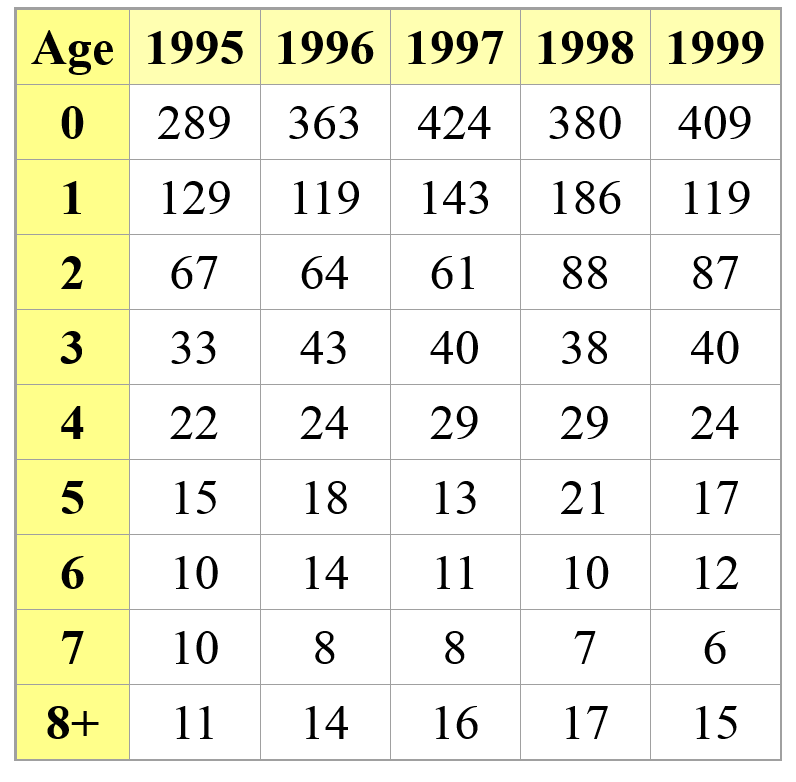
\includegraphics{figures/census1.png}

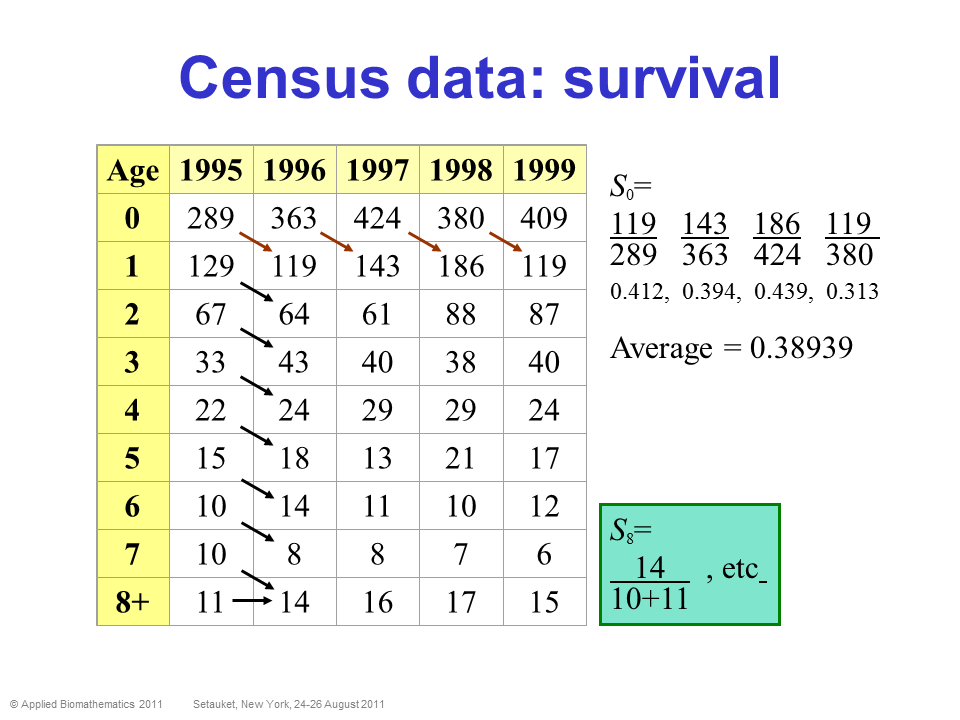
\includegraphics{figures/census2.png}

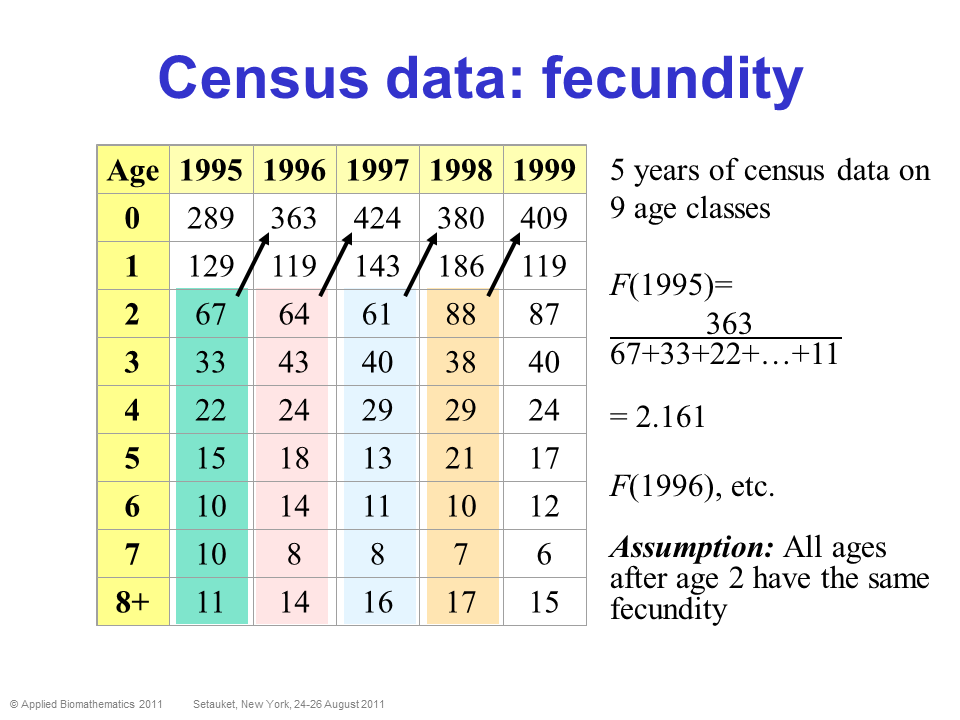
\includegraphics{figures/census3.png}

\textbf{PROS} - Puede estimar la supervivencia y la fecundidad, env.
estocasticidad, dependencia de la densidad, ¡prácticamente todo lo que
queremos para un modelo de población!

\begin{itemize}
\tightlist
\item
  Muy raramente (si es que alguna vez) disponible !!
\item
  Ignora la ** detección imperfecta ** (asume una detección perfecta),
  que casi siempre no es realista.
\end{itemize}

\hypertarget{capture-mark-recapture-cmr}{%
\subsubsection{Capture-mark-recapture
(CMR)}\label{capture-mark-recapture-cmr}}

\textbf{PROS} - Puede estimar supervivencia, variación en supervivencia,
lambda, reclutamiento, tasas de dispersión. - ¡Probablemente la fuente
de datos más utilizada para modelos de población!

\textbf{CONS} - Pocas desventajas, aunque las técnicas analíticas pueden
ser difíciles de dominar - Montar un estudio CMR adecuado puede resultar
muy costoso y requerir muchos años de datos. - La estimación de los
movimientos a escala del paisaje puede requerir un estudio aún más
costoso y que requiere más tiempo. - En muchos casos, la emigración y la
supervivencia pueden ser difíciles de separar.

¡Vea más abajo para más! Además, este es el enfoque principal del curso
de Dinámica de la población (NRES 488, ¡el próximo curso en la secuencia
de Ecología y Conservación de la Vida Silvestre!)

\hypertarget{datos-sobre-estructura-espacial-huxe1bitat}{%
\subsubsection{Datos sobre estructura espacial /
hábitat}\label{datos-sobre-estructura-espacial-huxe1bitat}}

\begin{itemize}
\tightlist
\item
  Vea \href{FINAL_PROJECTS.html}{links} en la página de proyectos
  finales
\end{itemize}

\hypertarget{quuxe9-pasa-si-no-hay-datos}{%
\subsubsection{¿Qué pasa si ``no hay
datos''?}\label{quuxe9-pasa-si-no-hay-datos}}

Recuerda el \href{https://en.wikipedia.org/wiki/Stone_Soup}{``Stone
Soup'' analogy!} - incluso cuando crea que no hay datos, ¡probablemente
haya más de los que parece inicialmente!

\begin{itemize}
\tightlist
\item
  Usar álgebra para construir una matriz de transición estructurada por
  edades completa a partir de la información disponible.

  \begin{itemize}
  \tightlist
  \item
    Por ejemplo, nos falta información sobre la supervivencia de las
    crías. Solo sabemos:

    \begin{itemize}
    \tightlist
    \item
      Tasas de supervivencia de jóvenes y adultos
    \item
      Éxito de anidación
    \item
      El crecimiento de la población (lambda) es 1.09
    \item
      ¡Ahora podemos resolver la supervivencia de las crías!
    \item
      Para un ejemplo de esto, ver {[}Congdon et al 1993{]} (congdon et
      al 1993.pdf)
    \end{itemize}
  \end{itemize}
\item
  ¡Simplifica! (Los modelos son siempre representaciones simplificadas
  de la realidad)

  \begin{itemize}
  \tightlist
  \item
    ¿Ignora la estructura de edad? (es decir, use el modelo escalar)
  \item
    ¿Ignora la dependencia de la densidad?
  \item
    Ignore las interacciones tróficas (¡generalmente hacemos esta
    simplificación de todos modos!)
  \item
    Ignorar la abundancia por completo (por ejemplo, utilizar el modelo
    de metapoblación clásico)
  \end{itemize}
\item
  Estrategias conservadoras (use * el peor de los casos *)!

  \begin{itemize}
  \tightlist
  \item
    El modelo independiente de la densidad es conservador, por lo que si
    no tiene datos en D-D, ¡tal vez simplemente ignórelo!
  \item
    Con incertidumbre de los parámetros, utilice el peor de los casos
  \item
    Bajo tendencias de declive, use el peor de los casos
  \end{itemize}
\item
  ¡Utilice datos de especies similares!

  \begin{itemize}
  \tightlist
  \item
    Por ejemplo, las especies de tamarinos tienen historias de vida
    similares, así que utilice datos sobre titíes león dorado para
    modelar los titíes león con cabeza dorada.
  \end{itemize}
\item
  Opinión experta

  \begin{itemize}
  \tightlist
  \item
    Vea abajo\ldots{}
  \end{itemize}
\item
  Bases de datos nacionales

  \begin{itemize}
  \tightlist
  \item
    Vea \href{FINAL_PROJECTS.html}{links} en la página de proyectos
    finales
  \end{itemize}
\item
  \href{https://www.astronomyclub.xyz/maternal-effect/does-ecology-have-laws.html}{Allometries}

  \begin{itemize}
  \tightlist
  \item
    por ejemplo, la alometría de Fenchel
  \item
    Este tipo de pensamiento (que busca patrones amplios entre especies)
    a menudo se denomina ``macroecología''.
  \end{itemize}
\end{itemize}

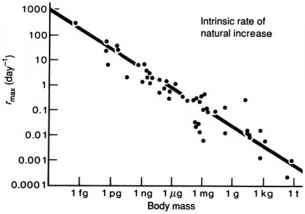
\includegraphics{figures/allometry2.jpg}

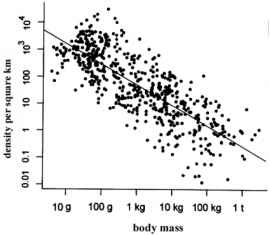
\includegraphics{figures/allometry1.jpg}

\hypertarget{aparte-se-puede-utilizar-la-opiniuxf3n-de-un-experto}{%
\subsection{Aparte, ¿se puede utilizar la opinión de un
experto?}\label{aparte-se-puede-utilizar-la-opiniuxf3n-de-un-experto}}

\begin{itemize}
\tightlist
\item
  No es ideal, porque es difícil o imposible de validar y difícil de
  documentar, pero \ldots{}
\item
  ¡Eso es lo que se hará en cualquier caso!
\item
  Y es mejor usarlo que no hacer nada
\item
  Y es mejor documentar que se utilizó la opinión de expertos que
  proceder con la planificación de la conservación en ausencia de
  fuentes y supuestos establecidos.
\item
  Es un punto de partida (y a veces uno razonable)
\end{itemize}

\hypertarget{anuxe1lisis-de-captura-marca-recaptura-cmr-capture-mark-recapture-cmr-analysis}{%
\subsection{Análisis de captura-marca-recaptura (CMR):
Capture-mark-recapture (CMR)
analysis}\label{anuxe1lisis-de-captura-marca-recaptura-cmr-capture-mark-recapture-cmr-analysis}}

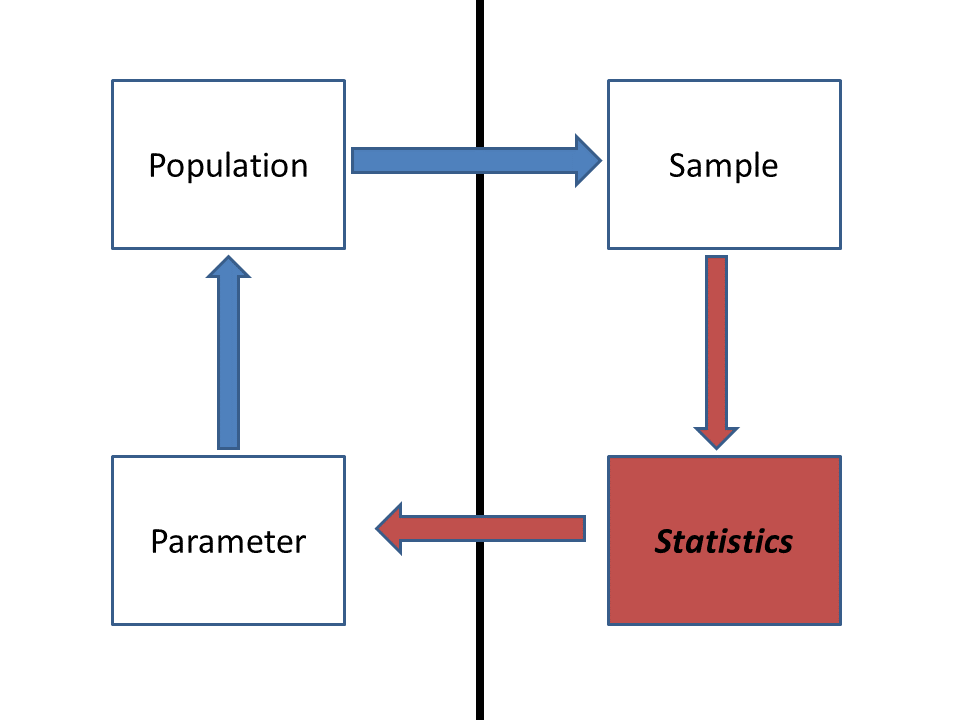
\includegraphics{figures/statistics1.png}

\hypertarget{paruxe1metros-pva-estimables-a-partir-de-datos-cmr}{%
\subsubsection{Parámetros PVA estimables a partir de datos
CMR}\label{paruxe1metros-pva-estimables-a-partir-de-datos-cmr}}

\begin{itemize}
\tightlist
\item
  Tasa de supervivencia (posiblemente estructurada por edad o tamaño)
\item
  Fecundidad (entrada de nuevos individuos en la población)
\item
  Reclutamiento (ingreso de nuevos individuos a la población adulta)
\item
  abundancia
\item
  Lambda (tasa de crecimiento finita)
\item
  Influencias ambientales en las tasas de supervivencia y fecundidad.
\item
  Varianza del proceso temporal (estocasticidad env.)
\item
  Tasas de dispersión
\end{itemize}

\hypertarget{los-datos-necesarios-para-el-anuxe1lisis-cmr-historiales-de-captura}{%
\subsubsection{Los datos necesarios para el análisis CMR: historiales de
captura}\label{los-datos-necesarios-para-el-anuxe1lisis-cmr-historiales-de-captura}}

Considere un proyecto diseñado para monitorear una población de
caimanes. Estos caimanes fueron monitoreados durante cuatro años, desde
1976 hasta 1979.

Cada fila de la siguiente tabla representa un historial de capturas
posible único:

Un ``1'' indica que un animal fue capturado con éxito en un año
determinado y posteriormente liberado.

Un ``0'' indica que un animal no fue capturado con éxito en un año
determinado.

Un ``2'' indica que un animal fue capturado con éxito en un año
determinado, pero no fue devuelto a la población (probablemente murió
debido a la manipulación o captura).

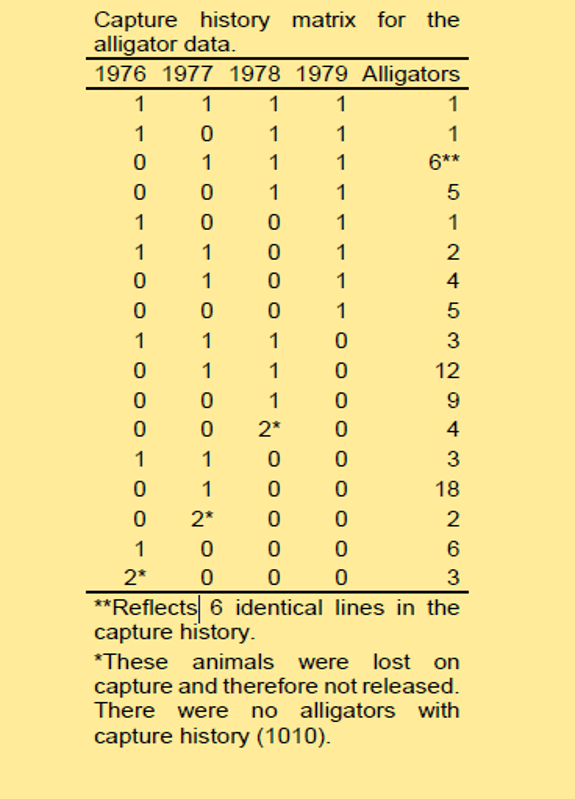
\includegraphics{figures/caphist1.png}

\hypertarget{dos-tipos-principales-de-anuxe1lisis-cmr}{%
\subsubsection{Dos tipos principales de análisis
CMR}\label{dos-tipos-principales-de-anuxe1lisis-cmr}}

\hypertarget{modelos-poblacionales-cerrados}{%
\paragraph{Modelos poblacionales
cerrados}\label{modelos-poblacionales-cerrados}}

Suponemos que la población está cerrada (¡sin procesos BIDE!). Es decir,
¡la abundancia no cambia! ¡Intentamos estimar la abundancia!

\begin{itemize}
\tightlist
\item
  Sin mortalidad
\item
  Sin nacimientos
\item
  Sin inmigración
\item
  Sin emigración
\item
  Todos los individuos son observables (pero no necesariamente
  observados \ldots)
\end{itemize}

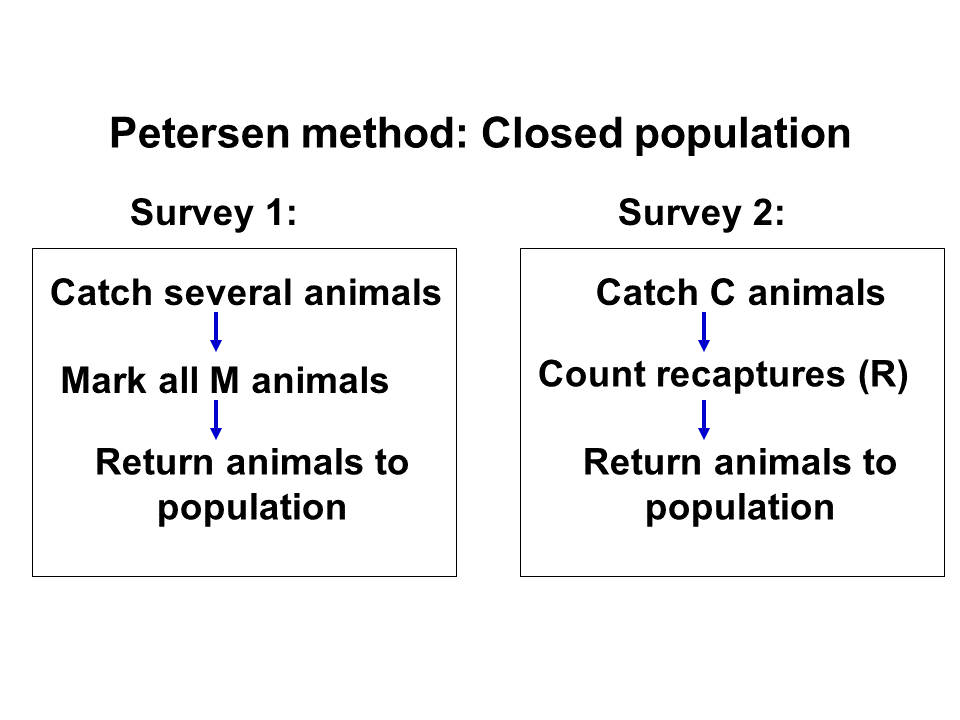
\includegraphics{figures/peterson1.png}

Parámetros estimados:

\begin{itemize}
\tightlist
\item
  abundancia
\end{itemize}

M = el número de individuos marcados en la primera muestra C = número
total de individuos capturados en la segunda muestra R = número de
individuos en la segunda muestra que están marcados

Podemos usar la siguiente fórmula para estimar la abundancia (el
\textbf{estimador lincoln-peterson }):

\(N = \frac{M \times C}{R}\)

\hypertarget{modelos-de-poblaciuxf3n-abiertos}{%
\paragraph{Modelos de población
abiertos}\label{modelos-de-poblaciuxf3n-abiertos}}

Suponemos que la población está abierta a uno o más de los procesos
BIDE. Es decir, ¡la abundancia PUEDE cambiar! Intentamos estimar los
procesos que impulsan el cambio de abundancia (a menudo, tasas de
supervivencia)

\begin{itemize}
\tightlist
\item
  Poblaciones abiertas al nacimiento, la muerte y posiblemente incluso
  la migración (la abundancia puede cambiar durante el estudio).
\item
  Permite la estimación de los impulsores de la dinámica de la población
  durante períodos de tiempo prolongados
\item
  A menudo de gran interés para ecologistas y gestores.
\end{itemize}

\hypertarget{muxe1xima-verosimilitud-un-marco-para-la-inferencia-estaduxedstica}{%
\subsubsection{Máxima verosimilitud: ¡un marco para la inferencia
estadística!}\label{muxe1xima-verosimilitud-un-marco-para-la-inferencia-estaduxedstica}}

\textbf{PARA ANÁLISIS CMR }: - ¿Qué valor de supervivencia maximiza la
probabilidad de generar los historiales de captura observados?

EJEMPLO:

Considere el siguiente historial de captura de una sola persona:

\begin{verbatim}
1 0 1 1
\end{verbatim}

Este individuo fue marcado y liberado en la captura inicial. No se
capturó en la siguiente encuesta, pero luego se capturó en cada una de
las siguientes dos encuestas posteriores.

¿Cuál es la probabilidad de observar este historial de capturas?

\begin{quote}
{[}(Probabilidad de sobrevivir del tiempo 1 al 2) X (Probabilidad de no
ser visto en el momento 2){]} X {[}(Probabilidad de sobrevivir del
tiempo 2 al 3) X (Probabilidad de ser visto en el momento 3){]} X
{[}(Probabilidad de sobrevivir del tiempo 3 al 4) X (Probabilidad de ser
visto en el tiempo 4){]}
\end{quote}

-\textgreater{} {[}(Probability of surviving from time 1 to 2) X
(Probability of not being seen at time 2){]} X {[}(Probability of
surviving from time 2 to 3) X (Probability of being seen at time 3){]} X
{[}(Probability of surviving from time 3 to 4) X (Probability of being
seen at time 4){]}

Esto se puede escribir:

\(L_1 = \phi_1(1-p_2) \cdot \phi_2p_3 \cdot \phi_3p_4\)

¿Qué tal el siguiente historial de captura para una sola persona?

\begin{verbatim}
1 0 1 0
\end{verbatim}

¿Cuál es la probabilidad de observar este historial de capturas?

\begin{quote}
{[}(Probabilidad de sobrevivir del tiempo 1 al 2) X (Probabilidad de no
ser visto en el momento 2){]} X {[}(Probabilidad de sobrevivir del
tiempo 2 al 3) X (Probabilidad de ser visto en el momento 3){]} X
\end{quote}

-\textgreater{} {[}(Probability of surviving from time 1 to 2) X
(Probability of not being seen at time 2){]} X {[}(Probability of
surviving from time 2 to 3) X (Probability of being seen at time 3){]} X

-- either --

\begin{quote}
{[}(Probability of surviving from time 3 to 4) X (Probability of not
being seen at time 4){]}
\end{quote}

-- or --

\begin{quote}
{[}(Probability of NOT surviving from time 3 to 4)
\end{quote}

Esto se puede escribir:

\(L_1 = \phi_1(1-p_2) \cdot \phi_2p_3 \cdot \left \{(1-\phi_3)+\phi_3(1-p_4) \right \}\)

\textbf{P }: si la supervivencia fuera del 100\% y la probabilidad de
captura fuera del 100\%, ¿cuál es la probabilidad de observar los
historiales de captura anteriores?

\textbf{P }: ¿y si la supervivencia fuera del 100\% y la probabilidad de
captura fuera del 75\%?

La estimación de máxima verosimilitud es el proceso de encontrar los
valores de los parámetros \$ ~phi \$ y \$ p \$ que serían más *
probables * para generar los historiales de captura observados.

Este modelo se conoce como el modelo \emph{Cormack-Jolly-Seber } (CJS) y
es el análisis más común realizado por el programa MARK.

*P **: ¿Por qué \$ ~phi \$ también se conoce como supervivencia
``aparente''? ¿Por qué no es la ``verdadera'' supervivencia ???

\hypertarget{supuestos-clave-del-modelo-cjs}{%
\paragraph{Supuestos clave del modelo
CJS}\label{supuestos-clave-del-modelo-cjs}}

\begin{itemize}
\tightlist
\item
  Todos los individuos de la población son igualmente detectables en
  cada ocasión de muestreo (cada sesión de captura representa una
  muestra totalmente aleatoria de la población)
\item
  Los topógrafos no pierden ni pierden las marcas
\item
  Toda emigración es permanente (equivalente a una mortalidad)
\end{itemize}

\hypertarget{program-mark}{%
\subsubsection{Program MARK}\label{program-mark}}

MARK es un motor numérico de máxima verosimilitud diseñado para el
análisis de marcado-recaptura. Ingresa un conjunto de datos del
historial de captura y MARK generará resultados como la tasa de
supervivencia y la probabilidad de captura.

\hypertarget{ejemplo-de-un-anuxe1lisis-de-marcado-recaptura-de-poblaciuxf3n-abierta}{%
\subsection{¡Ejemplo de un análisis de marcado-recaptura de población
abierta!}\label{ejemplo-de-un-anuxe1lisis-de-marcado-recaptura-de-poblaciuxf3n-abierta}}

¡Repasemos un análisis CJS en R! Para seguir adelante, por favor
\href{LECTURE15.R}{guarde este script y cárguelo en Rstudio}.

NOTA: este análisis incluye tanto hombres como mujeres (a diferencia del
ejemplo del laboratorio 7), por lo que los resultados se verán algo
diferentes.

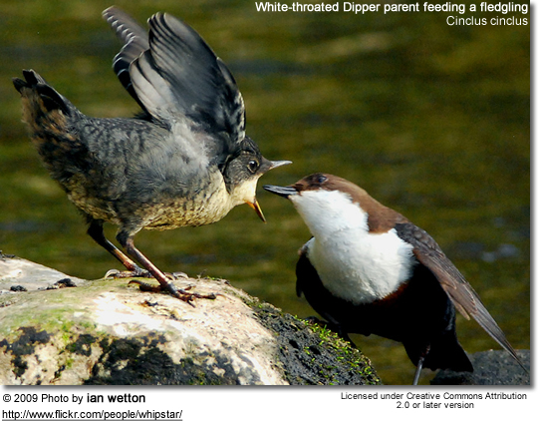
\includegraphics{figures/dipper1.png}

Los datos del cazo europeo son EL ejemplo clásico de un conjunto de
datos CMR. ¡Veámos!

\begin{Shaded}
\begin{Highlighting}[]
\DocumentationTok{\#\#\#\#\#\#\#\#\#\#\#}
\CommentTok{\# Cormack{-}Jolly{-}Seber (CJS) model in R}
\DocumentationTok{\#\#\#\#\#\#\#\#\#\#\#}

\FunctionTok{library}\NormalTok{(marked)      }\CommentTok{\# install the \textquotesingle{}marked\textquotesingle{} package if you haven\textquotesingle{}t already done this!}
\FunctionTok{data}\NormalTok{(}\StringTok{"dipper"}\NormalTok{)}
\FunctionTok{head}\NormalTok{(dipper,}\DecValTok{10}\NormalTok{)}
\end{Highlighting}
\end{Shaded}

\begin{verbatim}
##         ch    sex
## 1  0000001 Female
## 2  0000001 Female
## 3  0000001 Female
## 4  0000001 Female
## 5  0000001 Female
## 6  0000001 Female
## 7  0000001 Female
## 8  0000001 Female
## 9  0000001 Female
## 10 0000001 Female
\end{verbatim}

Aquí usamos el paquete ``marked'' en R (en lugar de MARK) para hacer la
estimación del parámetro ML.

\begin{Shaded}
\begin{Highlighting}[]
\DocumentationTok{\#\#\#\#\#\#\#\#\#\#}
\CommentTok{\# load data!}

\FunctionTok{data}\NormalTok{(dipper)}

\DocumentationTok{\#\#\#\#\#\#\#\#\#\#\#\#\#}
\CommentTok{\# Process data}

\NormalTok{dipper.proc}\OtherTok{=}\FunctionTok{process.data}\NormalTok{(dipper,}\AttributeTok{model=}\StringTok{"cjs"}\NormalTok{,}\AttributeTok{begin.time=}\DecValTok{1}\NormalTok{)  }\CommentTok{\# Helper function{-} process the data for CJS model}
\end{Highlighting}
\end{Shaded}

\begin{verbatim}
## 255 capture histories collapsed into 53
\end{verbatim}

\begin{Shaded}
\begin{Highlighting}[]
\NormalTok{dipper.ddl}\OtherTok{=}\FunctionTok{make.design.data}\NormalTok{(dipper.proc)    }\CommentTok{\# another helper function{-} process data!}

\DocumentationTok{\#\#\#\#\#\#\#\#\#\#}
\CommentTok{\# Fit models}

\CommentTok{\# fit time{-}varying cjs model}


\FunctionTok{capture.output}\NormalTok{(}\FunctionTok{suppressMessages}\NormalTok{(   }\CommentTok{\# note: this is just to suppress messages to avoid cluttering the website...}
\NormalTok{      mod.Phit.pt }\OtherTok{\textless{}{-}}  \FunctionTok{crm}\NormalTok{(dipper.proc,dipper.ddl,}\AttributeTok{model.parameters=}\FunctionTok{list}\NormalTok{(}\AttributeTok{Phi=}\FunctionTok{list}\NormalTok{(}\AttributeTok{formula=}\SpecialCharTok{\textasciitilde{}}\NormalTok{time),}\AttributeTok{p=}\FunctionTok{list}\NormalTok{(}\AttributeTok{formula=}\SpecialCharTok{\textasciitilde{}}\NormalTok{time)),}\AttributeTok{method=}\StringTok{"Nelder{-}Mead"}\NormalTok{,}\AttributeTok{hessian =}\NormalTok{ T)}
\NormalTok{),}\AttributeTok{file=}\StringTok{"temp.txt"}\NormalTok{) }

\NormalTok{mod.Phit.pt   }\CommentTok{\# print out model}
\end{Highlighting}
\end{Shaded}

\begin{verbatim}
## 
## crm Model Summary
## 
## Npar :  12
## -2lnL:  657.0644
## AIC  :  681.0644
## 
## Beta
##                    Estimate        se        lcl       ucl
## Phi.(Intercept)  0.75646636 0.6570806 -0.5314116 2.0443444
## Phi.time2       -0.99255899 0.7541098 -2.4706142 0.4854962
## Phi.time3       -0.84151202 0.6991672 -2.2118797 0.5288557
## Phi.time4       -0.22522075 0.7051952 -1.6074034 1.1569619
## Phi.time5       -0.36893542 0.6974964 -1.7360284 0.9981576
## Phi.time6        0.10115137 1.5063624 -2.8513189 3.0536216
## p.(Intercept)    1.00571207 0.8006508 -0.5635635 2.5749876
## p.time3          1.49463757 1.3119503 -1.0767850 4.0660601
## p.time4          1.37853596 1.0927336 -0.7632220 3.5202939
## p.time5          1.12053506 0.9914942 -0.8227937 3.0638638
## p.time6          1.57229762 1.0715540 -0.5279483 3.6725435
## p.time7          0.07823848 1.7821210 -3.4147187 3.5711956
\end{verbatim}

\begin{Shaded}
\begin{Highlighting}[]
\NormalTok{mod.Phit.pt}\SpecialCharTok{$}\NormalTok{results}\SpecialCharTok{$}\NormalTok{AIC       }\CommentTok{\# extract AIC}
\end{Highlighting}
\end{Shaded}

\begin{verbatim}
## [1] 681.0644
\end{verbatim}

\begin{Shaded}
\begin{Highlighting}[]
\DocumentationTok{\#\#\#\#\#\#\#\#}
\CommentTok{\# fit time{-}invariant cjs model}

\FunctionTok{capture.output}\NormalTok{(}\FunctionTok{suppressMessages}\NormalTok{(}
\NormalTok{  mod.Phidot.pdot }\OtherTok{\textless{}{-}} \FunctionTok{crm}\NormalTok{(dipper.proc,dipper.ddl,}\AttributeTok{model.parameters =} \FunctionTok{list}\NormalTok{(}\AttributeTok{Phi=}\FunctionTok{list}\NormalTok{(}\AttributeTok{formula=}\SpecialCharTok{\textasciitilde{}}\DecValTok{1}\NormalTok{),}\AttributeTok{p=}\FunctionTok{list}\NormalTok{(}\AttributeTok{formula=}\SpecialCharTok{\textasciitilde{}}\DecValTok{1}\NormalTok{)),}\AttributeTok{method=}\StringTok{"Nelder{-}Mead"}\NormalTok{,}\AttributeTok{hessian =} \ConstantTok{TRUE}\NormalTok{)}
\NormalTok{),}\AttributeTok{file=}\StringTok{"temp.txt"}\NormalTok{)}

\NormalTok{mod.Phidot.pdot}
\end{Highlighting}
\end{Shaded}

\begin{verbatim}
## 
## crm Model Summary
## 
## Npar :  2
## -2lnL:  666.8377
## AIC  :  670.8377
## 
## Beta
##                  Estimate        se        lcl       ucl
## Phi.(Intercept) 0.2422903 0.1020150 0.04234102 0.4422397
## p.(Intercept)   2.2261889 0.3251153 1.58896300 2.8634148
\end{verbatim}

\begin{Shaded}
\begin{Highlighting}[]
\NormalTok{mod.Phidot.pdot}\SpecialCharTok{$}\NormalTok{results}\SpecialCharTok{$}\NormalTok{AIC}
\end{Highlighting}
\end{Shaded}

\begin{verbatim}
## [1] 670.8377
\end{verbatim}

\begin{Shaded}
\begin{Highlighting}[]
\DocumentationTok{\#\#\#\#\#\#\#\#}
\CommentTok{\# fit sex{-}dependent cjs model}

\FunctionTok{capture.output}\NormalTok{(}\FunctionTok{suppressMessages}\NormalTok{(}
\NormalTok{  mod.Phisex.psex }\OtherTok{\textless{}{-}} \FunctionTok{crm}\NormalTok{(dipper.proc,dipper.ddl,}\AttributeTok{model.parameters =} \FunctionTok{list}\NormalTok{(}\AttributeTok{Phi=}\FunctionTok{list}\NormalTok{(}\AttributeTok{formula=}\SpecialCharTok{\textasciitilde{}}\NormalTok{sex),}\AttributeTok{p=}\FunctionTok{list}\NormalTok{(}\AttributeTok{formula=}\SpecialCharTok{\textasciitilde{}}\NormalTok{sex)),}\AttributeTok{method=}\StringTok{"Nelder{-}Mead"}\NormalTok{,}\AttributeTok{hessian =} \ConstantTok{TRUE}\NormalTok{)}
\NormalTok{),}\AttributeTok{file=}\StringTok{"temp.txt"}\NormalTok{)}

\NormalTok{mod.Phisex.psex}
\end{Highlighting}
\end{Shaded}

\begin{verbatim}
## 
## crm Model Summary
## 
## Npar :  4
## -2lnL:  666.1518
## AIC  :  674.1518
## 
## Beta
##                   Estimate        se         lcl       ucl
## Phi.(Intercept) 0.22338784 0.1440981 -0.05904451 0.5058202
## Phi.sexMale     0.04138178 0.2041878 -0.35882631 0.4415899
## p.(Intercept)   2.01072100 0.4210671  1.18542943 2.8360126
## p.sexMale       0.47587463 0.6630165 -0.82363774 1.7753870
\end{verbatim}

\begin{Shaded}
\begin{Highlighting}[]
\NormalTok{mod.Phisex.psex}\SpecialCharTok{$}\NormalTok{results}\SpecialCharTok{$}\NormalTok{AIC}
\end{Highlighting}
\end{Shaded}

\begin{verbatim}
## [1] 674.1518
\end{verbatim}

\begin{Shaded}
\begin{Highlighting}[]
\DocumentationTok{\#\#\#\#\#\#\#\#\#\#\#}
\CommentTok{\# compare all models with AIC}
\DocumentationTok{\#\#\#\#\#\#\#\#\#\#\#}

\DocumentationTok{\#\#\#\#\#\#}
\CommentTok{\# Set up models to run (must have either "Phi." or "p." in the name)}
\NormalTok{Phi.dot }\OtherTok{\textless{}{-}} \FunctionTok{list}\NormalTok{(}\AttributeTok{formula=}\SpecialCharTok{\textasciitilde{}}\DecValTok{1}\NormalTok{)       }
\NormalTok{Phi.time }\OtherTok{\textless{}{-}} \FunctionTok{list}\NormalTok{(}\AttributeTok{formula=}\SpecialCharTok{\textasciitilde{}}\NormalTok{time)}
\NormalTok{Phi.sex }\OtherTok{\textless{}{-}} \FunctionTok{list}\NormalTok{(}\AttributeTok{formula=}\SpecialCharTok{\textasciitilde{}}\NormalTok{sex)}
\NormalTok{Phi.timesex }\OtherTok{\textless{}{-}} \FunctionTok{list}\NormalTok{(}\AttributeTok{formula=}\SpecialCharTok{\textasciitilde{}}\NormalTok{sex}\SpecialCharTok{+}\NormalTok{time)}
\NormalTok{p.dot }\OtherTok{\textless{}{-}} \FunctionTok{list}\NormalTok{(}\AttributeTok{formula=}\SpecialCharTok{\textasciitilde{}}\DecValTok{1}\NormalTok{)}
\NormalTok{p.time }\OtherTok{\textless{}{-}} \FunctionTok{list}\NormalTok{(}\AttributeTok{formula=}\SpecialCharTok{\textasciitilde{}}\NormalTok{time)}
\NormalTok{p.sex }\OtherTok{\textless{}{-}} \FunctionTok{list}\NormalTok{(}\AttributeTok{formula=}\SpecialCharTok{\textasciitilde{}}\NormalTok{sex)}
\NormalTok{p.timesex }\OtherTok{\textless{}{-}} \FunctionTok{list}\NormalTok{(}\AttributeTok{formula=}\SpecialCharTok{\textasciitilde{}}\NormalTok{sex}\SpecialCharTok{+}\NormalTok{time)}

\NormalTok{cml}\OtherTok{=}\FunctionTok{create.model.list}\NormalTok{(}\FunctionTok{c}\NormalTok{(}\StringTok{"Phi"}\NormalTok{,}\StringTok{"p"}\NormalTok{))    }\CommentTok{\# create list of all models to run}

\DocumentationTok{\#\#\#\#\#\#}
\CommentTok{\# Run all models}

\FunctionTok{capture.output}\NormalTok{(}\FunctionTok{suppressMessages}\NormalTok{(}\FunctionTok{suppressWarnings}\NormalTok{(}
\NormalTok{  allmodels }\OtherTok{\textless{}{-}} \FunctionTok{crm.wrapper}\NormalTok{(cml,}\AttributeTok{data=}\NormalTok{dipper.proc, }\AttributeTok{ddl=}\NormalTok{dipper.ddl,}\AttributeTok{external=}\ConstantTok{FALSE}\NormalTok{,}\AttributeTok{accumulate=}\ConstantTok{FALSE}\NormalTok{,}\AttributeTok{method=}\StringTok{"Nelder{-}Mead"}\NormalTok{,}\AttributeTok{hessian=}\ConstantTok{TRUE}\NormalTok{)}
\NormalTok{)),}\AttributeTok{file=}\StringTok{"temp.txt"}\NormalTok{)}

\DocumentationTok{\#\#\#\#\#\#}
\CommentTok{\# AIC model selection}

\NormalTok{allmodels}
\end{Highlighting}
\end{Shaded}

\begin{verbatim}
##                             model npar      AIC  DeltaAIC       weight  neg2lnl
## 1                    Phi(~1)p(~1)    2 670.8377  0.000000 0.3792707172 666.8377
## 2                  Phi(~1)p(~sex)    3 672.1934  1.355756 0.1925531715 666.1934
## 5                  Phi(~sex)p(~1)    3 672.6762  1.838541 0.1512568696 666.6762
## 9                 Phi(~time)p(~1)    7 673.7301  2.892463 0.0893015564 659.7301
## 6                Phi(~sex)p(~sex)    4 674.1518  3.314151 0.0723253541 666.1518
## 10              Phi(~time)p(~sex)    8 675.1913  4.353613 0.0430104833 659.1913
## 13          Phi(~sex + time)p(~1)    8 675.6617  4.824056 0.0339952989 659.6617
## 14        Phi(~sex + time)p(~sex)    9 677.1681  6.330419 0.0160072363 659.1681
## 3                 Phi(~1)p(~time)    7 678.4804  7.642778 0.0083050299 664.4804
## 4           Phi(~1)p(~sex + time)    8 679.9497  9.112045 0.0039837661 663.9497
## 7               Phi(~sex)p(~time)    8 680.4921  9.654404 0.0030375415 664.4921
## 11             Phi(~time)p(~time)   12 681.0644 10.226756 0.0022815888 657.0644
## 12       Phi(~time)p(~sex + time)   13 681.7032 10.865580 0.0016577483 655.7032
## 8         Phi(~sex)p(~sex + time)    9 681.8896 11.051978 0.0015102292 663.8896
## 15       Phi(~sex + time)p(~time)   13 682.9670 12.129303 0.0008812611 656.9670
## 16 Phi(~sex + time)p(~sex + time)   14 683.6633 12.825655 0.0006221479 655.6633
##    convergence
## 1            0
## 2            0
## 5            0
## 9            0
## 6            0
## 10           0
## 13           0
## 14           0
## 3            0
## 4            0
## 7            0
## 11           0
## 12           0
## 8            0
## 15           0
## 16           1
\end{verbatim}

\begin{Shaded}
\begin{Highlighting}[]
\DocumentationTok{\#\#\#\#\#\#\#}
\CommentTok{\# get parameter estimates and confidence intervals for best model}

\NormalTok{allmodels[[}\DecValTok{1}\NormalTok{]]}
\end{Highlighting}
\end{Shaded}

\begin{verbatim}
## 
## crm Model Summary
## 
## Npar :  2
## -2lnL:  666.8377
## AIC  :  670.8377
## 
## Beta
##                  Estimate        se        lcl       ucl
## Phi.(Intercept) 0.2422903 0.1020150 0.04234102 0.4422397
## p.(Intercept)   2.2261889 0.3251153 1.58896300 2.8634148
\end{verbatim}

\begin{Shaded}
\begin{Highlighting}[]
\NormalTok{allmodels[[}\DecValTok{11}\NormalTok{]]}
\end{Highlighting}
\end{Shaded}

\begin{verbatim}
## 
## crm Model Summary
## 
## Npar :  12
## -2lnL:  657.0644
## AIC  :  681.0644
## 
## Beta
##                    Estimate        se        lcl       ucl
## Phi.(Intercept)  0.75646636 0.6570806 -0.5314116 2.0443444
## Phi.time2       -0.99255899 0.7541098 -2.4706142 0.4854962
## Phi.time3       -0.84151202 0.6991672 -2.2118797 0.5288557
## Phi.time4       -0.22522075 0.7051952 -1.6074034 1.1569619
## Phi.time5       -0.36893542 0.6974964 -1.7360284 0.9981576
## Phi.time6        0.10115137 1.5063624 -2.8513189 3.0536216
## p.(Intercept)    1.00571207 0.8006508 -0.5635635 2.5749876
## p.time3          1.49463757 1.3119503 -1.0767850 4.0660601
## p.time4          1.37853596 1.0927336 -0.7632220 3.5202939
## p.time5          1.12053506 0.9914942 -0.8227937 3.0638638
## p.time6          1.57229762 1.0715540 -0.5279483 3.6725435
## p.time7          0.07823848 1.7821210 -3.4147187 3.5711956
\end{verbatim}

\begin{Shaded}
\begin{Highlighting}[]
\DocumentationTok{\#\#\#\#\#\#\#}
\CommentTok{\# make predictions and plot them. }

\FunctionTok{predict}\NormalTok{(allmodels[[}\DecValTok{1}\NormalTok{]])}\SpecialCharTok{$}\NormalTok{Phi}
\end{Highlighting}
\end{Shaded}

\begin{verbatim}
##   occ estimate         se       lcl       ucl
## 1   6 0.560278 0.02513307 0.5105837 0.6087926
\end{verbatim}

\begin{Shaded}
\begin{Highlighting}[]
\NormalTok{Phi\_by\_year }\OtherTok{\textless{}{-}} \FunctionTok{predict}\NormalTok{(allmodels[[}\DecValTok{11}\NormalTok{]])}\SpecialCharTok{$}\NormalTok{Phi    }\CommentTok{\# predict Phi for all years (based on the best Phi(t) model)}

\FunctionTok{suppressWarnings}\NormalTok{( }\FunctionTok{suppressMessages}\NormalTok{( }\FunctionTok{library}\NormalTok{(Hmisc,}\AttributeTok{quietly =}\NormalTok{ T) ))    }\CommentTok{\#load Hmisc package{-} has a nice error bar function}
\FunctionTok{plot}\NormalTok{(}\DecValTok{1}\SpecialCharTok{:}\FunctionTok{nrow}\NormalTok{(Phi\_by\_year),Phi\_by\_year}\SpecialCharTok{$}\NormalTok{estimate,}\AttributeTok{xlab=}\StringTok{"Year"}\NormalTok{,}\AttributeTok{ylab=}\StringTok{"Survival"}\NormalTok{,}\AttributeTok{ylim=}\FunctionTok{c}\NormalTok{(}\DecValTok{0}\NormalTok{,}\DecValTok{1}\NormalTok{),}\AttributeTok{main=}\StringTok{"Variability in Survival, dipper demo"}\NormalTok{)}
\FunctionTok{errbar}\NormalTok{(}\DecValTok{1}\SpecialCharTok{:}\FunctionTok{nrow}\NormalTok{(Phi\_by\_year),Phi\_by\_year}\SpecialCharTok{$}\NormalTok{estimate,Phi\_by\_year}\SpecialCharTok{$}\NormalTok{ucl,Phi\_by\_year}\SpecialCharTok{$}\NormalTok{lcl,}\AttributeTok{add=}\NormalTok{T)}
\end{Highlighting}
\end{Shaded}

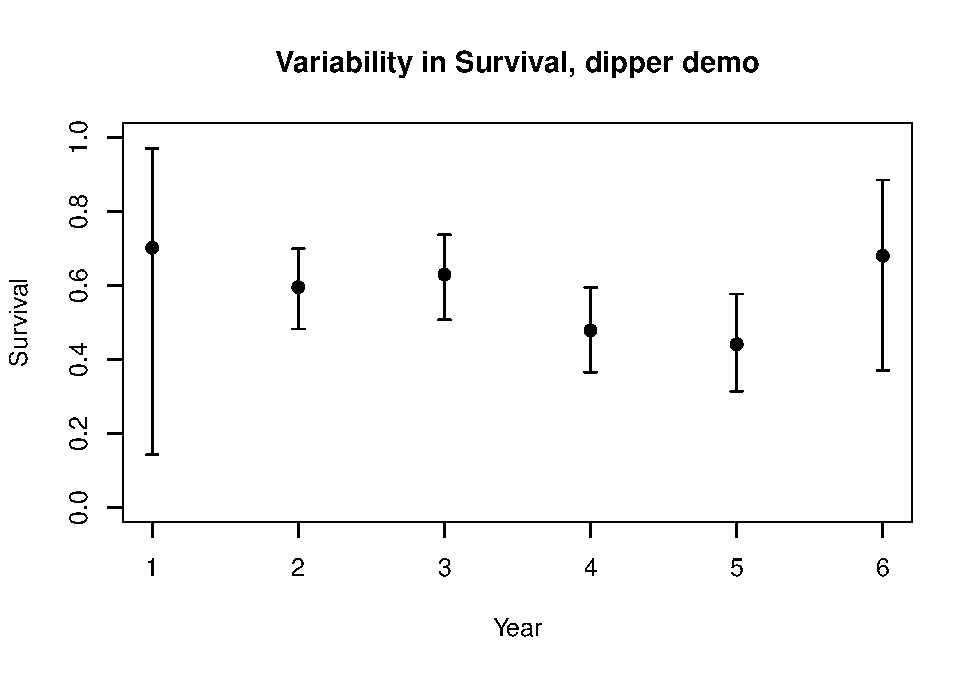
\includegraphics{LECTURE15_files/figure-latex/unnamed-chunk-5-1.pdf}

¿Cuál es nuestra estimación de supervivencia media?

\begin{Shaded}
\begin{Highlighting}[]
\DocumentationTok{\#\#\#\#\#\#\#}
\CommentTok{\# Calcule la tasa de supervivencia media de la población.}

\FunctionTok{mean}\NormalTok{(Phi\_by\_year}\SpecialCharTok{$}\NormalTok{estimate)}
\end{Highlighting}
\end{Shaded}

\begin{verbatim}
## [1] 0.5880352
\end{verbatim}

¿Qué es la estocasticidad ambiental?

\begin{Shaded}
\begin{Highlighting}[]
\DocumentationTok{\#\#\#\#\#\#\#}
\CommentTok{\# Calcule la variabilidad ambiental en las tasas de supervivencia anuales.}

\FunctionTok{sd}\NormalTok{(Phi\_by\_year}\SpecialCharTok{$}\NormalTok{estimate)}
\end{Highlighting}
\end{Shaded}

\begin{verbatim}
## [1] 0.1066587
\end{verbatim}

\hypertarget{program-mark-1}{%
\subsubsection{Program MARK!}\label{program-mark-1}}

MARK es un software gratuito y se puede descargar
desde\href{http://warnercnr.colostate.edu/~gwhite/mark/mark.htm}{here}

La demostración de Lab 7 se puede encontrar
\href{LAB7.html\#open-population_models}{here}

\href{LECTURE16.html}{--go to next lecture--}

\end{document}
